% ------------------------------------------------------------------------------
% TYPO3 CMS 8.5 - What's New - Chapter "Introduction" (German Version)
%
% @author	Michael Schams <schams.net>
% @license	Creative Commons BY-NC-SA 3.0
% @link		http://typo3.org/download/release-notes/whats-new/
% @language	English
% ------------------------------------------------------------------------------
% LTXE-CHAPTER-UID:		7fdf26cc-362160ab-d6c8b905-19722b20
% LTXE-CHAPTER-NAME:	Introduction
% ------------------------------------------------------------------------------

\section{Einführung}
\begin{frame}[fragile]
	\frametitle{Introduction}

	\begin{center}\huge{Einführung}\end{center}
	\begin{center}\huge{\color{typo3darkgrey}\textbf{Die Fakten}}\end{center}

\end{frame}

% ------------------------------------------------------------------------------
% LTXE-SLIDE-START
% LTXE-SLIDE-UID:		93bec580-20349d84-75d767fc-9ea5266e
% LTXE-SLIDE-ORIGIN:	344cc625-72176049-0721f1aa-0580f11a English
% LTXE-SLIDE-TITLE:		TYPO3 CMS 8.5 - The Facts
% ------------------------------------------------------------------------------
\begin{frame}[fragile]
	\frametitle{Introduction}
	\framesubtitle{TYPO3 CMS 8.5 - Die Fakten}

	\begin{itemize}
		\item Veröffentlichungsdatum: 20. Dezember 2016
		\item Releasetyp: Sprint Release
		\item Vision: On the clock
	\end{itemize}

	\begin{figure}
		
\includegraphics[width=0.95\linewidth]{Introduction/typo3cms85-banner.jpg}
	\end{figure}

\end{frame}

% ------------------------------------------------------------------------------
% LTXE-SLIDE-START
% LTXE-SLIDE-UID:		da07824b-8e47f465-17b29a4b-b3dd4c4d
% LTXE-SLIDE-ORIGIN:	59b04868-09a761b3-0c7ca4c3-ce6e31bb English
% LTXE-SLIDE-TITLE:		System Requirements
% ------------------------------------------------------------------------------
\begin{frame}[fragile]
	\frametitle{Introduction}
	\framesubtitle{Systemvoraussetzungen}

	\begin{itemize}
		\item PHP:\tabto{2.2cm}Version 7
		\item MySQL:\tabto{2.2cm}Version 5.5 bis 5.7
		\item Festplattenplatz:\tabto{2.2cm}min 200 MB
		\item PHP-Einstellungen:

			\begin{itemize}
				\item \texttt{memory\_limit} >= 128M
				\item \texttt{max\_execution\_time} >= 240s
				\item \texttt{max\_input\_vars} >= 1500
				\item Die Compile-Option \texttt{-}\texttt{-disable-ipv6} darf \underline{nicht} verwendet werden
			\end{itemize}

		\item Das Backend benötigt Microsoft Internet Explorer >= 11, Microsoft Edge, Google Chrome, Firefox, Safari oder jeden anderen modernen, kompatiblen Browser

	\end{itemize}

\end{frame}

% ------------------------------------------------------------------------------
% LTXE-SLIDE-START
% LTXE-SLIDE-UID:		43fa57f5-7bd287a9-9c56ccf8-3757ab3b
% LTXE-SLIDE-ORIGIN:	41f1b51a-6b837f9d-c4aa9584-66f8e47f English
% LTXE-SLIDE-TITLE:		Development And Release Timeline
% ------------------------------------------------------------------------------
\begin{frame}[fragile]
	\frametitle{Introduction}
	\framesubtitle{Release-Zyklus}

	\begin{figure}
		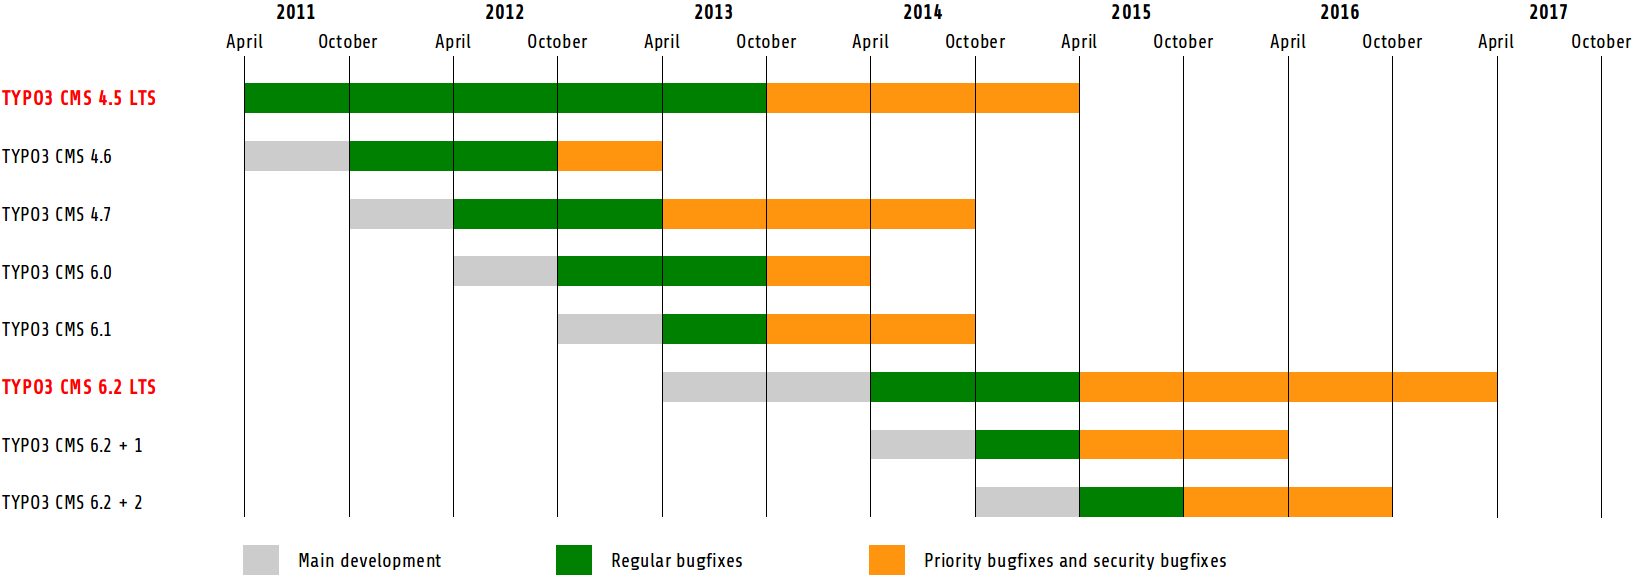
\includegraphics[width=1\linewidth]{Introduction/ReleaseAgenda.png}
	\end{figure}

\end{frame}

% ------------------------------------------------------------------------------
% LTXE-SLIDE-START
% LTXE-SLIDE-UID:		549480e8-8db54696-ef95503a-fffd19fd
% LTXE-SLIDE-ORIGIN:	f7c981ac-f359aac8-f8799a73-2adc6532 English
% LTXE-SLIDE-TITLE:		TYPO3 CMS Roadmap
% ------------------------------------------------------------------------------
\begin{frame}[fragile]
	\frametitle{Introduction}
	\framesubtitle{TYPO3 CMS Roadmap}

	Voraussichtliche Veröffentlichungen und deren Hauptfokus:

	\begin{itemize}

		\item v8.0 \tabto{1.0cm}22. März 2016\tabto{4.2cm}Adding last minute things
		\item v8.1 \tabto{1.0cm}03. Mai 2016\tabto{4.2cm}Cloud Integration
		\item v8.2 \tabto{1.0cm}05. Juli 2016\tabto{4.2cm}Doctrine Prerequisites
		\item v8.3 \tabto{1.0cm}30. August 2016\tabto{4.2cm}Rich Text Editor
		\item v8.4 \tabto{1.0cm}18. Oktober 2016\tabto{4.2cm}Doctrine Migration + Upgrades
		\item
			\begingroup
				\color{typo3orange}
					v8.5 \tabto{1.0cm}20. Dezember 2016\tabto{4.2cm}New RTE + Integrator Support
			\endgroup
		\item v8.6 \tabto{1.0cm}14. Februar 2017\tabto{4.2cm}\textit{to be determined}
		\item v8.7 \tabto{1.0cm}04. April 2017\tabto{4.2cm}LTS Vorbereitung

	\end{itemize}

	\smaller
		\url{https://typo3.org/typo3-cms/roadmap/}\newline
		\url{https://typo3.org/news/article/kicking-off-typo3-v8-development/}
	\normalsize

\end{frame}

% ------------------------------------------------------------------------------
% LTXE-SLIDE-START
% LTXE-SLIDE-UID:		d784a83f-83a9408a-f39bd9c8-0a095dcf
% LTXE-SLIDE-ORIGIN:	425f3f15-1178ed7e-f26438f9-a79ad9e9 English
% LTXE-SLIDE-TITLE:		Installation
% ------------------------------------------------------------------------------
\begin{frame}[fragile]
	\frametitle{Introduction}
	\framesubtitle{Installation}

	\begin{itemize}
		\item Empfohlene Installationsschritte unter Linux/Mac OS X\newline
			(DocumentRoot ist beispielsweise \texttt{/var/www/site/htdocs}):
		\begin{lstlisting}
			$ cd /var/www/site
			$ wget --content-disposition get.typo3.org/8.5
			$ tar xzf typo3_src-8.5.1.tar.gz
			$ cd htdocs
			$ ln -s ../typo3_src-8.5.1 typo3_src
			$ ln -s typo3_src/index.php
			$ ln -s typo3_src/typo3
			$ touch FIRST_INSTALL
		\end{lstlisting}

		\item Symbolische Links unter Microsoft Windows:

			\begin{itemize}
				\item unter Windows XP/2000 kann \texttt{junction} benutzt werden
				\item unter Windows Vista und Windows 7 kann \texttt{mklink} benutzt werden
			\end{itemize}

	\end{itemize}
\end{frame}

% ------------------------------------------------------------------------------
% LTXE-SLIDE-START
% LTXE-SLIDE-UID:		75bb6934-4ed7586b-4daa93d2-5412cbbb
% LTXE-SLIDE-ORIGIN:	061ecffe-6aadad2d-6e64a67a-3c50a5cf English
% LTXE-SLIDE-TITLE:		Upgrade to TYPO3 CMS 7
% ------------------------------------------------------------------------------
\begin{frame}[fragile]
	\frametitle{Introduction}
	\framesubtitle{Upgrade zu TYPO3 CMS 8.x}

	\begin{itemize}
		\item Upgrades sind nur möglich von TYPO3 CMS 7.6 LTS oder 8.x
		\item TYPO3 CMS < 7.6 LTS sollten zunächst auf TYPO3 CMS 7.6 LTS aktualisiert werden
	\end{itemize}

	\begin{itemize}

		\item Upgrade-Anleitung:\newline
			\smaller\url{http://wiki.typo3.org/Upgrade#Upgrading_to_8.5}\normalsize
		\item Offizielles TYPO3 Guide "TYPO3 Installation and Upgrading":
			\smaller\url{http://docs.typo3.org/typo3cms/InstallationGuide}\normalsize
		\item Generelles Vorgehen:
			\begin{itemize}
				\item Prüfen, ob Mindestvoraussetzungen erfüllt sind \small(PHP, MySQL, etc.)
				\item Das \textbf{deprecation\_*.log} der TYPO3 Instanz durchsehen
				\item Sämtliche Extensions auf den aktuellsten Stand bringen
				\item Neuen TYPO3 Quellcode entpacken und im Install Tool den Upgrade Wizard ausführen
				\item Startup Modul von Backend Benutzern überprüfen (optional)
			\end{itemize}
	\end{itemize}

\end{frame}


% ------------------------------------------------------------------------------
% LTXE-SLIDE-START
% LTXE-SLIDE-UID:		7a839525-a5683524-ede87801-d63e0acd
% LTXE-SLIDE-ORIGIN:	560abc87-898d82d3-b9e35f84-e348c121 English
% LTXE-SLIDE-TITLE:		PHP Version 7
% ------------------------------------------------------------------------------
\begin{frame}[fragile]
	\frametitle{Introduction}
	\framesubtitle{PHP Version 7}

	\begin{itemize}

		\item PHP 7.0 ist die minimal mögliche Version für TYPO3 CMS 8.x
		\item TYPO3 wird kontinuierlich weitere PHP 7 Releases unterstützen, sobald diese veröffentlicht werden
		\item Diese Version beschleunigt das gesamte System signifikant

		\item Nicht nur Backend-Redakteure werden das deutlich beschleunigte Interface bemerken, auch der Aufruf des Caches im Frontend ist nun unter 7ms möglich, was ein Geschwindigkeitswachstum von 40\% gegenüber PHP 5.5 bedeutet

		\item Zeitgleicht wurden neue PHP 7 Features in den Core integriert, wie beispielsweise die Verwendung der kryptografischen Pseudo-Zufalls-Generatoren

	\end{itemize}

\end{frame}

% ------------------------------------------------------------------------------
